%!TEX root = ../deepsmooth.tex

\section{Results} \label{sec:results}

The first part presents results on synthetic data where it is easier to study and compare model predictions.
The second part presents results on real-world data to modeling implied volatility surfaces extracted from S\&P500 options prices.
The synthetic and market data are described in Appendix~\ref{sec:datasynt} and~\ref{sec:datamkt} respectively.
We always set $\lambda_4=\lambda_5=\lambda_6=\lambda$ for some $\lambda\ge0$.


\subsection{Numerical experiments} \label{sec:numexp}

\begin{figure}
\centering
%\vspace{-0.3cm}
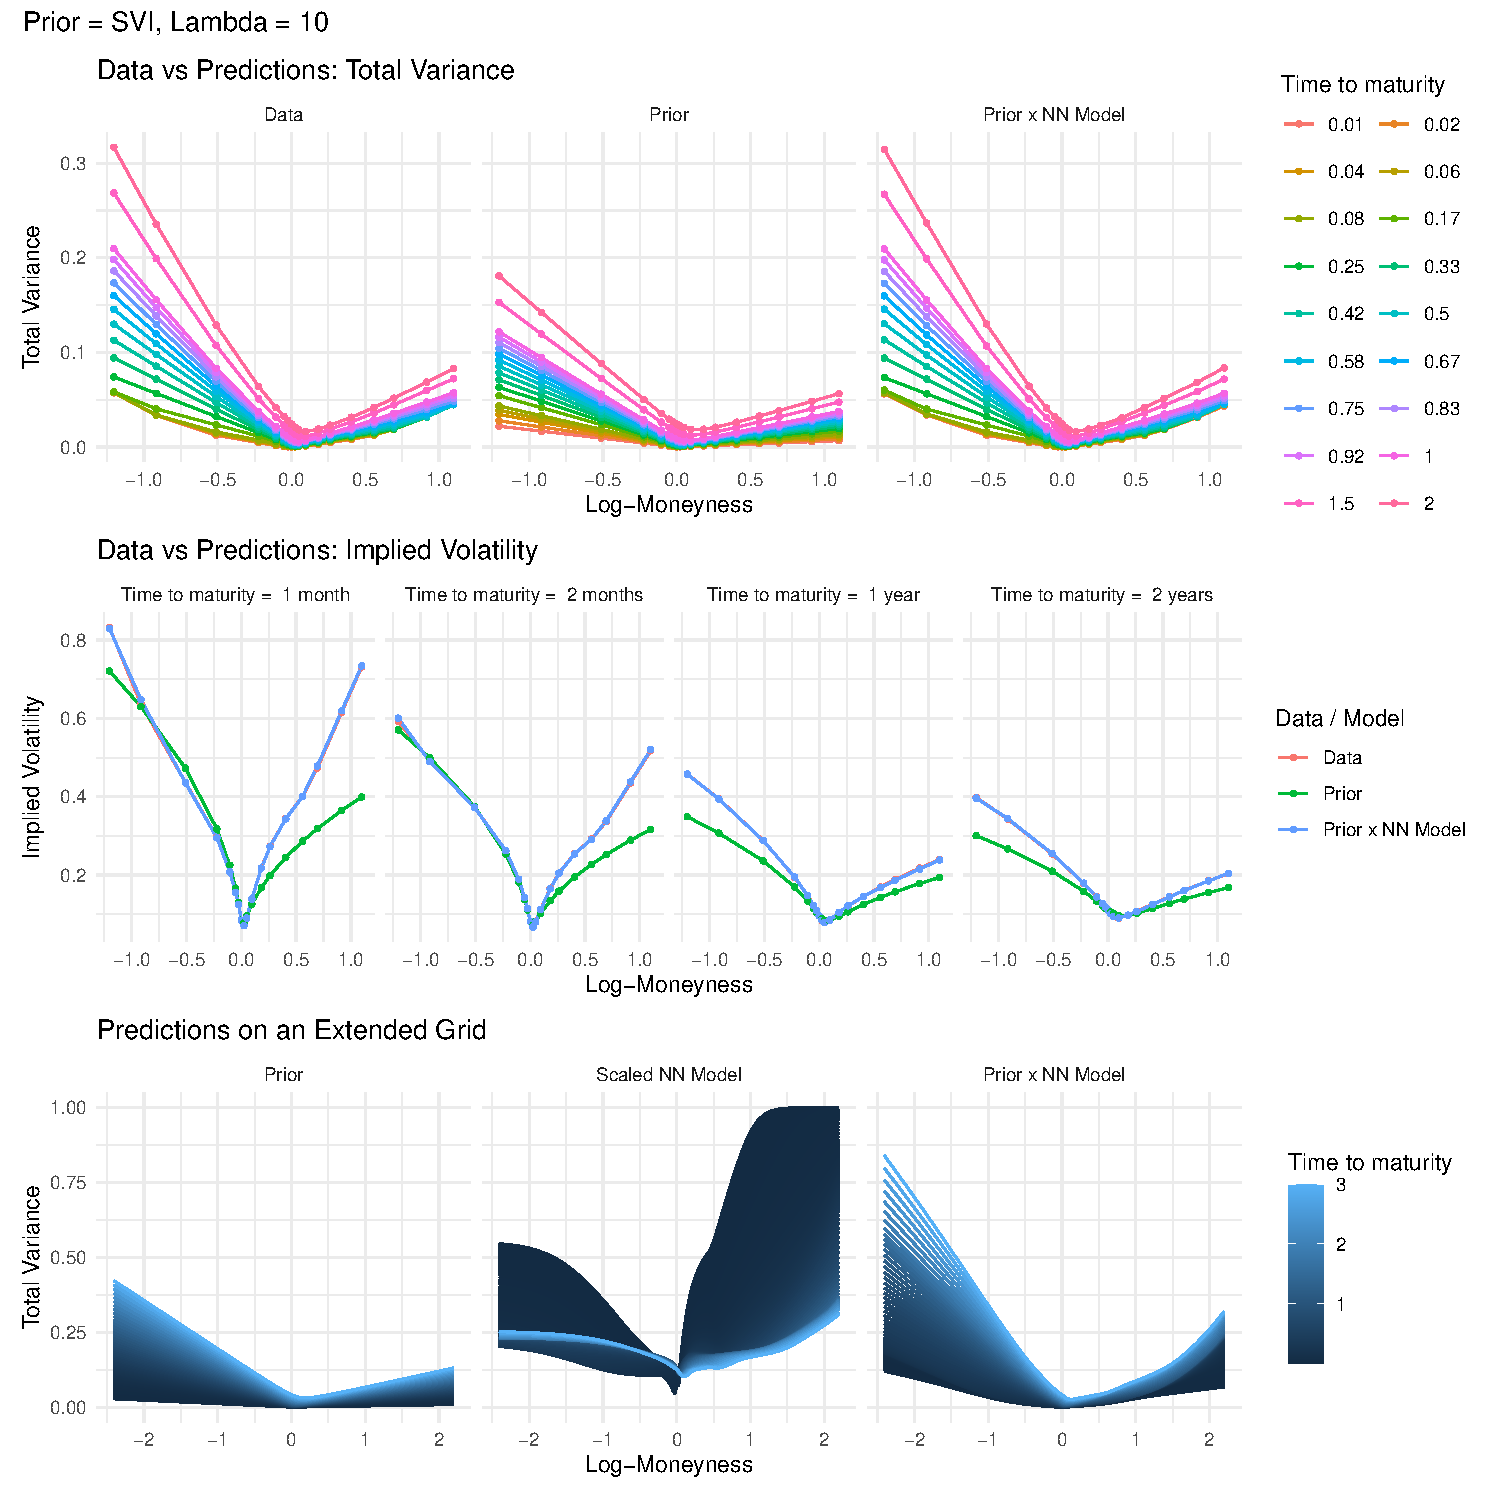
\includegraphics[width=\textwidth]{figures/numexp_fig12.pdf}
%\vspace{-0.4cm}
\caption{\label{fig:smoothsynt} Synthetic data and trained model predictions for a specific configuration (scenario 12).}
%\vspace{-0.4cm}
\end{figure}

\textbf{Smoothing behavior.}
\Cref{fig:smoothsynt} displays the trained model on synthetic data with a strong penalty $\lambda=10$.
A dot indicates the positioning $(k,\tau)$ of an observation used for training on figures in the top row.
The figures on the first and second rows show that $\ivpr$ does not succeed to reproduce the training data, while $\ivth$ does so perfectly.
The figures in the last row display $\ivpr$ and $\ivth$ on an extended grid of log moneyness, and also shows the NN correction before the scaling by $\alpha$ (center figure).
As $\ivpr$ fits at the money (ATM) term structure, $\ivth$ makes little correction to it on the region $k\approx0$.
On the other hand, $\ivth$ makes important corrections to $\ivpr$ for out of the money options.

The same figure for additional scenarios ($\lambda$ value, prior model, and data limits) can be found in Appendix~\ref{sec:smoothsynt}.
These additional results show that the model generalization is significantly better with a SSVI prior and with soft-constraints.
Indeed, the IVS tends to flatten for large log moneyness values with a BS prior, whereas the present data is V shaped.
Also, it is shown that the absence of soft-constraints can translate into non-realistic and possibly absurd out of sample predictions.


%% OLD TEXT
%A major challenge is the extrapolation of the implied volatility surface to unobserved data points.
%Flexible non-parametric methods typically fail as they lack the guidance of a parametric model.
%In \Cref{fig:smoothing} we calibrate ANN models with different loss terms and parameters initialization on a subsample of 100 options with narrow moneyness on the synthetic Bates data. 
%The three models fit the training set almost perfectly.
%Yet, we see that the ANN without arbitrage losses, $\lambda_4=\lambda_5=0$, fails extrapolate in a nonsensical way.
%On the other hand the arbitrage-free model with $\lambda_4=\lambda_5=10$ behaves very smoothly.
%The last model is initialized with the weights of an ANN model fitted to a Bates model itself fitted on the training set, see Appendix~B.3.
%It is furthermore penalized so that its weights remain close to its initialization weights with $\lambda_3=1$.
%This confirms that a regularized learning can produce an extrapolation mimicking the Bates model, with most notable differences in this example for the positive log-moneynesses.

%\begin{figure}
%  \centering
%  \input{figures/smoothing}
%  \vspace{-0.8cm}
%\caption{Extrapolation with different loss specification and weights initialization.\label{fig:smoothing}}
%\end{figure}


\textbf{Losses and convergence.}

\Cref{fig:convsvi} displays statistics on the losses in~\eqref{eq:loss} for trained models with different number of layers, neurons per layer, and penalty value $\lambda$.
A total of 50 models with different random seeds for parameter initialization have been trained for 5'000 epochs for each configuration.
Recall that, with $\lambda=x$, the weight on the soft constraints is $x$ times larger than the loss on the predictions errors.
We see that increasing the number of layers or of neurons per layers generally decreases the RMSE and MAPE.
We also see that the arbitrage opportunities vanish as $\lambda$ increases.
The models prediction errors typically worsen as $\lambda$ increases, but the effect appears stronger for the lesser flexible models.
We also observe that, when the number of layers is smaller, increasing the neurons per layer without enforcing more strictly the constraints can generate more severe arbitrage opportunities.
But such opportunities disappear completely when the absence of arbitrage penalty is given a higher weight.
Additional results can be found in Appendix~\ref{sec:convergence} for the BS prior where,
in particular, we observe that the prediction errors are worse for this choice of prior model.

\begin{figure}
\centering
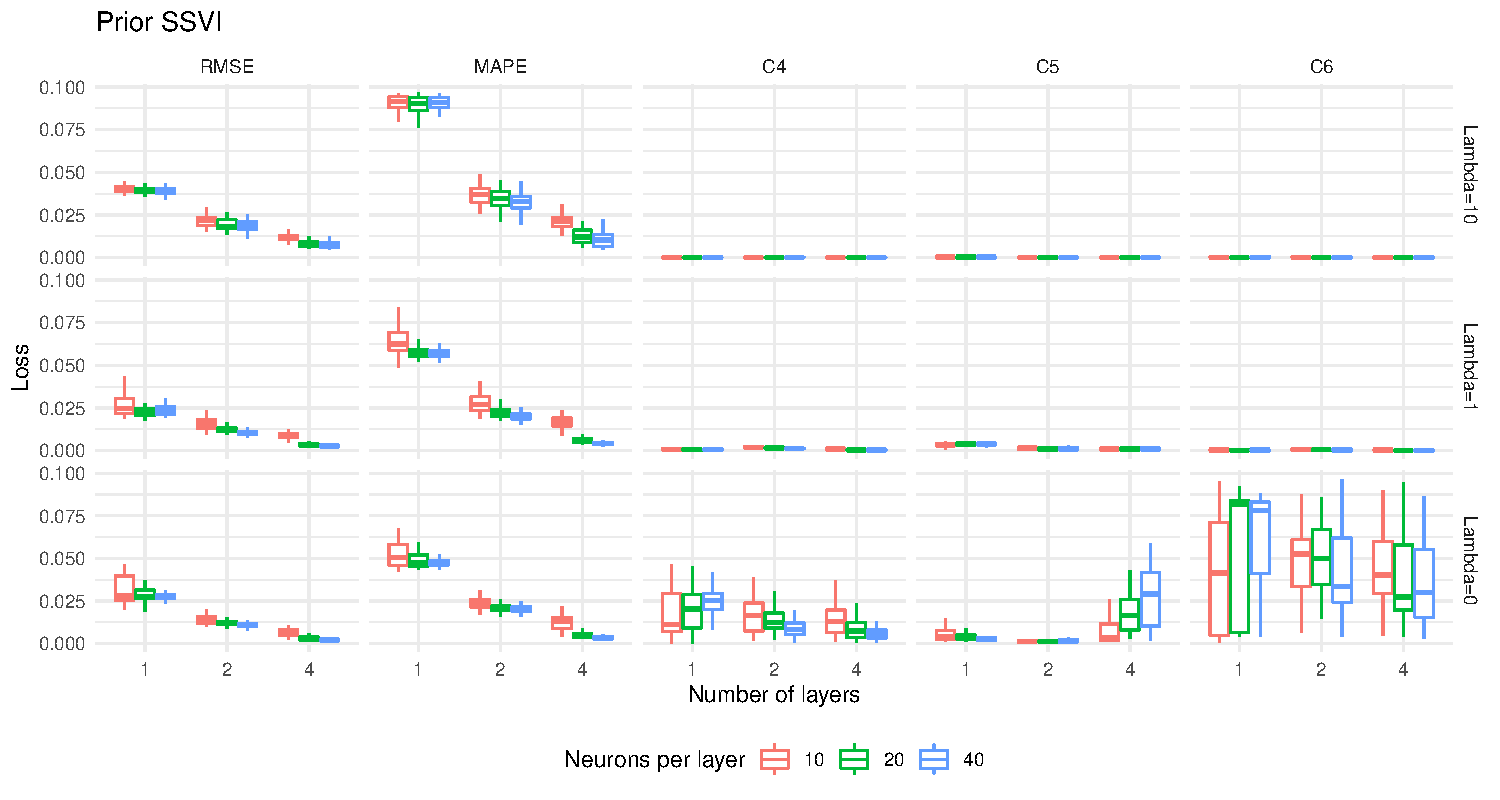
\includegraphics[width=\textwidth]{figures/numexp_nn_ssvi.pdf}
\caption{\label{fig:convsvi} Losses for different number of layers, neurons per layer, and penalty value.}
%\vspace{-0.2cm}
\end{figure}

\textbf{Additional results.}
In Appendix~\ref{sec:dugasetal} we show that the NN model suggested in~\cite{dugas2001incorporating} cannot capture the IVS on its full range of maturities and moneynesses for the synthetic data.
We also illustrate the impact of increasing arbitrage opportunities on the losses in Appendix~\ref{sec:numpexpao}.


\subsection{Empirical results} \label{sec:empres}


\textbf{Smoothing market data.}
\Cref{fig:smoothmkt} displays S\&P500 options data and trained model predictions with a strong penalty $\lambda=10$ for the April 13-th 2018.
This market data contains several thousands observations, and the corresponding IVS has a fairly complex shape compared to the previous synthetic data. 
The first two rows highlight that $\ivpr$ fails to reproduce the market data, but that $\ivth$ is able to make accurate predictions.
Notice that, because of data noise, the target IVS seem not to be arbitrage-free as some total variance slices cross each others, see upper-left figure.
Yet, the predictions generated by $\ivth$ are perfectly smooth and the slices do not cross.
The same figure for additional scenarios can be found in Appendix~\ref{sec:smoothmkt}.

\textbf{Backtests.}
We perform the following exercise for each day in the sample.
First, we split the daily sample into a training and a testing set.
Second, we fit the model on the training set and evaluate its performance on the testing set.
We use two different configurations for training and testing.
In the interpolation setting, for each maturity, we randomly select half of the contracts.
As such, we also sample options that are far out or in the money for training, and the testing error represents the approximation error for the range of moneyness that are actually observed.
In the extrapolation setting, for each maturity, we select half of the contracts whose log moneyness is between the 10\% and 90\% of the log moneyness in the corresponding slice.
This second filter therefore contains more observations around the money.
Thus, we do not select options that are far out or in the money for training, and the testing error measures how well our model extrapolates.
Finally, we again use three values for $\lambda$ in order to study how the arbitrage-related penalties affect the results.

In~\Cref{tab:bktSSVI} we present our results for model trained daily on the S\&P500 options data between January and April 2018, and for the subprime crisis period between September and December 2008, with a SSVI prior.
First, we describe the RMSE and MAPE.
As expected, training errors are generally below testing errors.
Increasing the no-arbitrage penalty $\lambda$ leads to worse RMSE and MAPE metrics on the training set.
However, larger $\lambda$ also implies similar or even less RMSE and MAPE metrics on the testing set.
Note that the RMSE for testing set of the extrapolation appears to be large compared to the MAPE.
The extrapolation errors are most of the time larger than interpolation errors.
This suggest that the high RMSE value is likely to be caused by deep out of the money options with large IV values.
Regarding \ref{cons:mono}--\ref{cons:asym}, we see that the models resulting from $\lambda=1,10$ are essentially arbitrage-free.
As for the model resulting from no enforcement of the constraints (i.e., $\lambda=0$), it generates arbitrage opportunities both in interpolation and extrapolation.
Note that 99+ indicates a value larger than 99 which can happen for arbitrage losses when $\lambda=0$.

Additional results for the BS prior, as well as for baselines models (Bates and SSVI models), can be found in Appendix~\ref{sec:backtests}.
Our approach surpasses the baseline models in terms of prediction accuracy, which should not be a surprise.
Indeed, in Section~\ref{sec:numexp} we showed that $\ivth$ could reproduce the IVS from a typical Bates model, hence it is likely to be at least as flexible.
In addition, $\ivth$ with a SSVI prior $\ivpr$ is likely to perform better than the underlying baseline SSVI model.

\begin{figure}
\centering
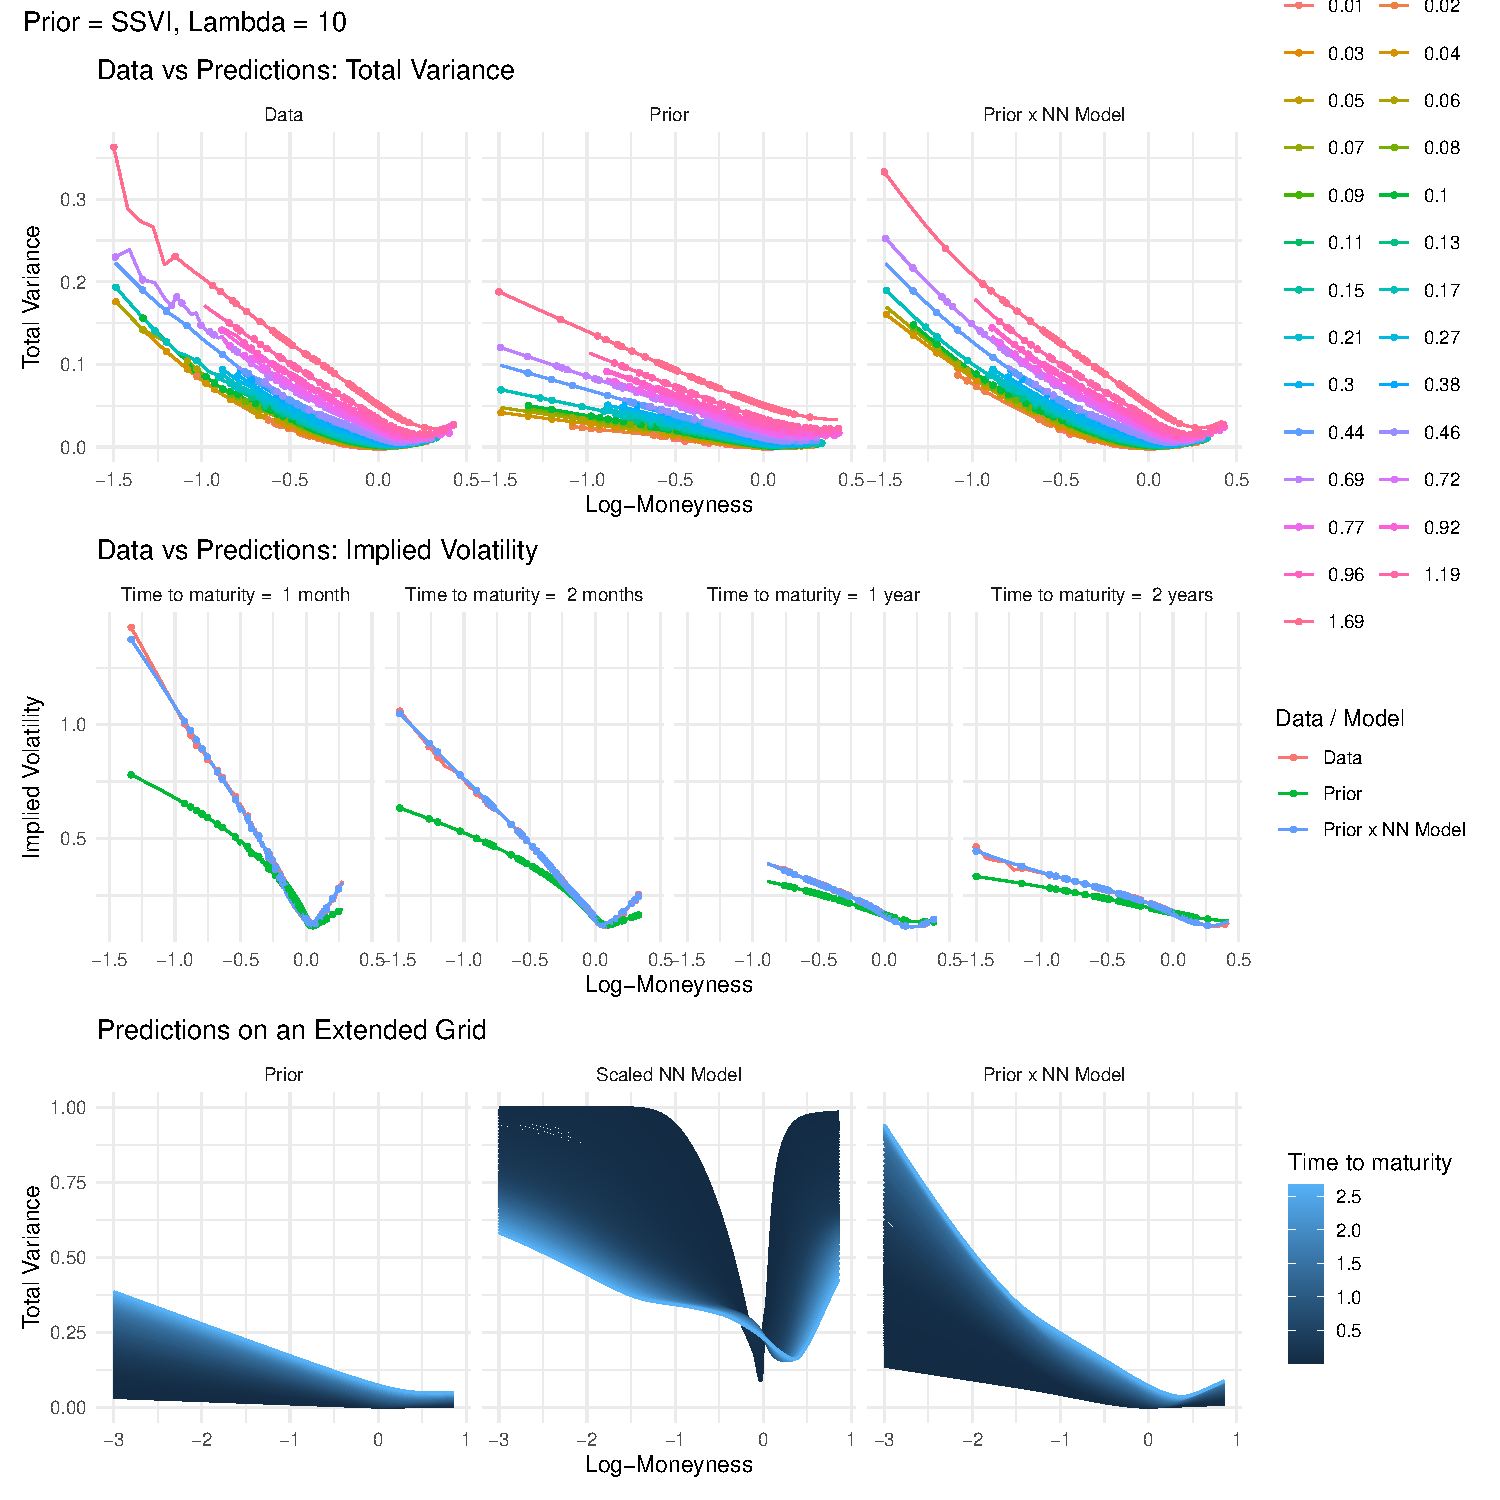
\includegraphics[width=\textwidth]{figures/empexp_fig12.pdf}
\caption{\label{fig:smoothmkt} Market data and trained model predictions for a specific configuration (scenario 12).}
\end{figure}

\begin{table}
\vspace{-0.5cm}
\caption{\label{tab:bktSSVI}Backtesting results for the SSVI prior (quantiles in \%, Jan-Apr 2018 / Sep-Dec 2008)}
\centering
\resizebox{\textwidth}{!}{
\begin{tabular}[t]{cccccccccccccc}
\toprule
\multicolumn{1}{c}{ } & \multicolumn{1}{c}{ } & \multicolumn{6}{c}{Interpolation} & \multicolumn{6}{c}{Extrapolation} \\
\cmidrule(l{3pt}r{3pt}){3-8} \cmidrule(l{3pt}r{3pt}){9-14}
\multicolumn{1}{c}{ } & \multicolumn{1}{c}{ } & \multicolumn{3}{c}{Train} & \multicolumn{3}{c}{Test} & \multicolumn{3}{c}{Train} & \multicolumn{3}{c}{Test} \\
\cmidrule(l{3pt}r{3pt}){3-5} \cmidrule(l{3pt}r{3pt}){6-8} \cmidrule(l{3pt}r{3pt}){9-11} \cmidrule(l{3pt}r{3pt}){12-14}
Loss & $\lambda$ & $q_{05}$ & $q_{50}$ & $q_{95}$ & $q_{05}$ & $q_{50}$ & $q_{95}$ & $q_{05}$ & $q_{50}$ & $q_{95}$ & $q_{05}$ & $q_{50}$ & $q_{95}$\\
\midrule
 & 10 & 0.4 / 0.7 & 0.5 / 3.1 & 1.3 / 19.9 & 0.4 / 0.9 & 0.5 / 3.3 & 1.4 / 18.8 & 0.2 / 0.3 & 0.3 / 1.1 & 0.4 / 3.5 & 2.2 / 2.7 & 5.0 / 6.3 & 8.0 / 12.0\\
\cmidrule{2-14}
 & 1 & 0.3 / 3.0 & 0.4 / 6.8 & 1.0 / 13.9 & 0.4 / 2.9 & 0.5 / 7.1 & 1.3 / 13.5 & 0.2 / 1.9 & 0.2 / 4.4 & 0.4 / 10.6 & 3.7 / 5.0 & 6.6 / 10.6 & 11.7 / 20.5\\
\cmidrule{2-14}
\multirow{-3}{*}{\centering\arraybackslash RMSE} & 0 & 0.2 / 0.4 & 0.3 / 1.3 & 0.5 / 4.0 & 0.3 / 1.6 & 0.5 / 3.5 & 4.8 / 10.8 & 0.2 / 0.3 & 0.2 / 0.9 & 0.3 / 3.3 & 3.1 / 5.5 & 7.5 / 11.6 & 18.1 / 26.7\\
\cmidrule{1-14}
 & 10 & 0.5 / 0.9 & 0.7 / 2.1 & 1.2 / 17.4 & 0.5 / 1.1 & 0.8 / 2.4 & 1.2 / 18.5 & 0.4 / 0.5 & 0.6 / 0.9 & 0.9 / 2.1 & 1.2 / 2.4 & 1.7 / 3.3 & 2.4 / 6.5\\
\cmidrule{2-14}
 & 1 & 0.5 / 4.0 & 0.6 / 8.2 & 1.2 / 12.2 & 0.5 / 4.3 & 0.7 / 8.1 & 1.3 / 12.9 & 0.3 / 2.2 & 0.5 / 6.3 & 0.9 / 11.0 & 1.5 / 5.6 & 2.3 / 9.7 & 3.3 / 13.1\\
\cmidrule{2-14}
\multirow{-3}{*}{\centering\arraybackslash MAPE} & 0 & 0.4 / 0.5 & 0.6 / 1.0 & 0.9 / 1.8 & 0.5 / 1.2 & 0.7 / 1.9 & 0.9 / 3.2 & 0.3 / 0.3 & 0.5 / 0.7 & 0.8 / 1.6 & 1.5 / 4.3 & 2.2 / 7.4 & 4.8 / 14.3\\
\cmidrule{1-14}
 & 10 & 0.0 / 0.0 & 0.0 / 0.0 & 0.0 / 0.2 & 0.0 / 0.0 & 0.0 / 0.0 & 0.0 / 0.5 & 0.0 / 0.0 & 0.0 / 0.0 & 0.0 / 0.0 & 0.0 / 0.0 & 0.0 / 0.0 & 0.0 / 14.1\\
\cmidrule{2-14}
 & 1 & 0.0 / 0.0 & 0.0 / 0.0 & 0.2 / 0.1 & 0.0 / 0.0 & 0.0 / 0.0 & 0.2 / 0.1 & 0.0 / 0.0 & 0.0 / 0.0 & 0.0 / 0.1 & 0.0 / 0.0 & 0.0 / 0.0 & 0.1 / 0.1\\
\cmidrule{2-14}
\multirow{-3}{*}{\centering\arraybackslash C4} & 0 & 1.6 / 1.5 & 18.0 / 9.8 & 99+ / 99+ & 1.6 / 1.2 & 40.7 / 12.1 & 99+ / 99+ & 0.3 / 1.1 & 2.4 / 3.7 & 44.2 / 83.7 & 0.4 / 1.0 & 2.8 / 4.3 & 46.7 / 30.4\\
\cmidrule{1-14}
 & 10 & 0.0 / 0.0 & 0.0 / 0.0 & 0.0 / 0.1 & 0.0 / 0.0 & 0.0 / 0.0 & 0.0 / 0.1 & 0.0 / 0.0 & 0.0 / 0.0 & 0.0 / 0.0 & 0.0 / 0.0 & 0.0 / 0.0 & 0.0 / 1.2\\
\cmidrule{2-14}
 & 1 & 0.0 / 0.0 & 0.0 / 0.0 & 0.1 / 0.0 & 0.0 / 0.0 & 0.0 / 0.0 & 0.5 / 0.0 & 0.0 / 0.0 & 0.0 / 0.0 & 0.0 / 0.0 & 0.0 / 0.0 & 0.0 / 0.0 & 0.5 / 0.0\\
\cmidrule{2-14}
\multirow{-3}{*}{\centering\arraybackslash C5} & 0 & 2.6 / 99+ & 72.1 / 99+ & 99+ / 99+ & 2.6 / 99+ & 63.8 / 99+ & 99+ / 99+ & 2.8 / 99+ & 24.2 / 99+ & 99+ / 99+ & 1.7 / 99+ & 19.0 / 99+ & 99+ / 99+\\
\cmidrule{1-14}
 & 10 & 0.0 / 0.0 & 0.0 / 0.0 & 0.0 / 0.2 & 0.0 / 0.0 & 0.0 / 0.0 & 0.0 / 0.6 & 0.0 / 0.0 & 0.0 / 0.0 & 0.0 / 0.0 & 0.0 / 0.0 & 0.0 / 0.0 & 0.0 / 44.3\\
\cmidrule{2-14}
 & 1 & 0.0 / 0.0 & 0.0 / 0.0 & 0.0 / 0.0 & 0.0 / 0.0 & 0.0 / 0.0 & 0.6 / 0.0 & 0.0 / 0.0 & 0.0 / 0.0 & 0.0 / 0.1 & 0.0 / 0.0 & 0.0 / 0.0 & 0.0 / 0.0\\
\cmidrule{2-14}
\multirow{-3}{*}{\centering\arraybackslash C6} & 0 & 0.8 / 0.0 & 48.2 / 1.7 & 99+ / 99+ & 0.8 / 0.0 & 78.4 / 0.4 & 99+ / 99+ & 0.3 / 0.1 & 12.0 / 7.5 & 99+ / 99+ & 0.0 / 0.0 & 2.4 / 0.0 & 99+ / 99+\\
\bottomrule
\end{tabular}
}
\end{table}



\textbf{Additional results.}
In Appendix~\ref{sec:pdflocvol} we display the risk-neutral density and the local volatility corresponding to the scenario 12.
The experience on Apple options in Appendix~\ref{sec:wshape} shows that our approach can fit complex shape surfaces, such as W-shaped smiles.
We trained a model on the absolute IV errors weighted by the IV spread in Appendix~\ref{sec:spreadw} which appears to converge faster but fails to learn the IVS shape far out of the money.
The computational times for the empirical experiments are reported in Appendix~\ref{sec:time} and appear satisfying despite the experimental nature of the implementation.

